\label{sec:05IdentifyGARCHmodel}
\section{Identify GARCH model}
\subsection{Using \textit{garchFit()} function and AIC}

In this section, we will try to fit the Residuals into a GARCH model due to the previous test proved that there are existing an ARCH Effect on the Residuals. Similar to fitting the ARMA Model, we will mainly rely on the AIC to search the (p,q) figures, which resulted in the smallest value then verify back with BIC.

By using the $garchFit()$ function and fitting with (p,q) $\in$ $\{1,2,..7\}$. We generated the table of AIC:

\FloatBarrier
\begin{table}[!htbp]
\centering
\begin{tabular}{|l||*{8}{c|}}\hline
\backslashbox{p}{q}
&\makebox[3em]{1}&\makebox[3em]{2}&\makebox[3em]{3}&\makebox[3em]{4}&\makebox[3em]{5}&\makebox[3em]{6}&\makebox[3em]{7} \\
\hline\hline
1 &-6.291084&-6.26150&-6.26064&-6.25907&-6.25752&-6.25595&-6.25559\\\hline
2 &-6.26127&-6.25996&-6.26006&-6.25850&-6.25695&-6.25655&-6.25490\\\hline
3 &-6.25971&-6.25840&-6.25986&-6.25833&-6.25678&-6.25522&-6.25366\\\hline
4 &-6.25815&-6.25684&-6.25833&-6.25676&-6.25521&-6.25366&-6.25210\\\hline
5 &-6.25699&-6.25634&-6.26142&-6.25986&-6.25830&-6.25677&-6.25521\\\hline
6 &-6.25538&-6.25564&-6.26005&-6.25859&-6.25708&-6.25552&-6.25397\\\hline
7 &-6.25618&-6.25552&-6.26022&-6.25705&-6.25569&-6.25413&-6.25256\\\hline
\end{tabular}
\caption{Table with AIC values}
\end{table}
\FloatBarrier
\FloatBarrier
\begin{figure}[!htbp]
  \centering
  \includegraphics[width=\textwidth]{img/Fig15.eps}
  \caption{Plotting the AIC generated with garchFit() function as (p,q) $\in \{1,2,...,7\}$}
\end{figure}
\FloatBarrier

We are now looking for the minimum AIC by running $which.mean()$ function for the table or simply spot out at the plotting, we can conclude that the minimum AIC resulted in GARCH Model with (p=1,q=1).

\subsection{Verify with BIC}

Furthermore, by using BIC result, we also got the same outcome which minimum BIC is equivalent to the GARCH model with (p=1,q=1). The results are shown in below table and graph. 

\FloatBarrier
\begin{table}[!htbp]
\centering
\begin{tabular}{|l||*{8}{c|}}\hline
\backslashbox{p}{q}
&\makebox[3em]{1}&\makebox[3em]{2}&\makebox[3em]{3}&\makebox[3em]{4}&\makebox[3em]{5}&\makebox[3em]{6}&\makebox[3em]{7} \\
\hline\hline
1 &-6.266921&-6.237335&-6.232446&-6.226852&-6.221281&-6.215684&-6.211287\\\hline
2 &-6.237109&-6.231772&-6.227842&-6.222252&-6.216677&-6.212248&-6.206579\\\hline
3 &-6.231522&-6.226187&-6.223615&-6.218056&-6.212478&-6.206895&-6.201307\\\hline
4 &-6.22593&-6.220594&-6.218056&-6.212467&-6.206888&-6.201305&-6.195718\\\hline
5 &-6.220749&-6.216066&-6.217119&-6.211536&-6.205946&-6.200396&-6.194806\\\hline
6 &-6.215109&-6.211338&-6.211722&-6.206236&-6.200701&-6.195111&-6.189535\\\hline
7 &-6.211882&-6.207192&-6.207866&-6.200673&-6.195284&-6.189694&-6.184105\\\hline
\end{tabular}
\caption{Table with BIC values}
\end{table}
\FloatBarrier

\FloatBarrier
\begin{figure}[!htbp]
  \centering
  \includegraphics[width=\textwidth]{img/Fig16.eps}
  \caption{Plotting the BIC generated with garchFit() function as (p,q) $\in \{1,2,...,7\}$}
\end{figure}
\FloatBarrier

\subsection{Parameters Estimation:}
\subsubsection{\textit{garchFit()} Function Details}
We estimate the parameter by $garchFit()$ function with Quasi Maximum Likelihood method:
\begin{lstlisting}[language=R]
garchFit(formula=(~arma(1,0)+garch(1,1)), 
	data=fit1$residuals,
        cond.dist="std")
\end{lstlisting}
We apply the Residuals data with ARMA(1,0), GARCH(1,1) and Student t-distribution.\\
\subsubsection{Result Outcome}
The fitting value as below:
\begin{lstlisting}[language=R]
Title:
 GARCH Modeling 

Call:
 garchFit(formula = (~arma(1, 0) + garch(1, 1)), data = fit1$residuals, 
    cond.dist = "std", trace = F) 

Mean and Variance Equation:
 data ~ arma(1, 0) + garch(1, 1)
<environment: 0x7f83d5ce5c00>
 [data = fit1$residuals]

Conditional Distribution:
 std 

Coefficient(s):
         mu          ar1        omega       alpha1        beta1        shape  
 3.3544e-04  -3.1853e-02   5.1781e-06   6.8382e-02   8.8838e-01   7.7848e+00  

Std. Errors:
 based on Hessian 

Error Analysis:
         Estimate  Std. Error  t value Pr(>|t|)    
mu      3.354e-04   2.736e-04    1.226  0.22017    
ar1    -3.185e-02   2.848e-02   -1.119  0.26332    
omega   5.178e-06   2.807e-06    1.844  0.06513 .  
alpha1  6.838e-02   2.227e-02    3.071  0.00214 ** 
beta1   8.884e-01   4.063e-02   21.865  < 2e-16 ***
shape   7.785e+00   1.574e+00    4.946 7.59e-07 ***
---

Log Likelihood:
 4032.293    normalized:  3.150229 

Description:
 Thu May 31 23:50:19 2018 by user:  


Standardised Residuals Tests:
                                Statistic p-Value     
 Jarque-Bera Test   R    Chi^2  103.9697  0           
 Shapiro-Wilk Test  R    W      0.9887748 2.411152e-08
 Ljung-Box Test     R    Q(10)  19.60848  0.03318098  
 Ljung-Box Test     R    Q(15)  22.55193  0.0941277   
 Ljung-Box Test     R    Q(20)  27.30132  0.1269975   
 Ljung-Box Test     R^2  Q(10)  10.65926  0.3846737   
 Ljung-Box Test     R^2  Q(15)  16.32737  0.3606346   
 Ljung-Box Test     R^2  Q(20)  23.51787  0.2640869   
 LM Arch Test       R    TR^2   12.66301  0.3940028   

Information Criterion Statistics:
      AIC       BIC       SIC      HQIC 
-6.291084 -6.266921 -6.291127 -6.282011 
\end{lstlisting}
\subsubsection{Interpret Coefficient}
We are fitting the ARMA(1,0)-GARCH(1,1) model with the following equation:
$$ Y_t = \varphi_1(Y_{t-1} - \mu) + \mu, $$
$$ \varepsilon_t = \sigma_t \eta_t, $$
$$ \sigma^2_t = \omega + \alpha_1 \varepsilon^2_{t-1},+ \beta_1\sigma^2_{t-1} $$
$$ \eta_t \sim Student(\gamma) $$
Matching with the $garchFit()$ coefficients output:

\FloatBarrier
\begin{table}[!htbp]
\centering
\begin{tabular}{|l|*{6}{c|}}
\hline
 $\mu$ & $\varphi_1$ & $\omega$ & $\alpha_1$ & $\beta_1$ & $\gamma$\\
 \hline
 mu & ar1 & omega & alpha1 & beta1 & shape\\
 \hline
 3.3544e-04 & -3.185e-02 & 5.178e-06 & 6.838e-02 & 8.884e-01 & 7.785\\
 \hline
\end{tabular}
\end{table}
\FloatBarrier

Then we have the CAC40 data from 2012 to 2017 can be model under ARMA(1,0) and the Residuals under GARCH(1,1) as below:
$$ r_t = -0.03185300(r_{t-1} - 0.00033544) + 0.00033544, $$
$$ \varepsilon_t = \sigma_t \eta_t, $$
$$ \sigma^2_t = 0.00000518 + 0.06838200 \varepsilon^2_{t-1},+ 0.88838000\sigma^2_{t-1} $$
$$ \varepsilon_t \sim Student(7.7848) $$

\subsection{GARCH Residual analysis}
We also do the GARCH Residual analysis via three steps, which are similar to the previous ARMA Residual Analysis. 

\subsubsection{GARCH Residual Plotting}
\FloatBarrier
\begin{figure}[!htbp]
  \centering
  \includegraphics[width=\textwidth]{img/Fig17.eps}
  \caption{Residuals Plot of GARCH(1,1)}
\end{figure}
\FloatBarrier
\FloatBarrier
\begin{figure}[!htbp]
  \centering
  \includegraphics[width=\textwidth]{img/Fig18.eps}
  \caption{Residuals Plot of GARCH(1,1)}
\end{figure}
\FloatBarrier
\subsubsection{Distribution Checking}
From the result of $garchFit()$ function in section 5.3.2:
\begin{lstlisting}[language=R]
Standardised Residuals Tests:
                                Statistic p-Value     
 Jarque-Bera Test   R    Chi^2  103.9697  0
 Shapiro-Wilk Test  R    W      0.9887748 2.411152e-08
\end{lstlisting}
We got the p-value is small in both Jarque-Bera Test \cite{jarque1980efficient} and Shapiro-Wilk Test \cite{royston1982extension}, which lead to the rejection of null hypothesis that the GARCH residuals are normally distributed.

\subsubsection{Autocorrelation Test}
From the result of $garchFit()$ function in section 5.3.2:
\begin{lstlisting}[language=R]
Standardised Residuals Tests:
                                Statistic p-Value     
 Ljung-Box Test     R    Q(10)  19.60848  0.03318098  
 Ljung-Box Test     R    Q(15)  22.55193  0.0941277   
 Ljung-Box Test     R    Q(20)  27.30132  0.1269975   
 Ljung-Box Test     R^2  Q(10)  10.65926  0.3846737   
 Ljung-Box Test     R^2  Q(15)  16.32737  0.3606346   
 Ljung-Box Test     R^2  Q(20)  23.51787  0.2640869     
 \end{lstlisting}
From the Ljung-Box Test \cite{box1970distribution,ljung1978measure} for both Residuals and Residuals Squared of GARCH(1,1), the p-value significantly higher than 0.05. That means we are unable to reject the null hypothesis that the GARCH residuals are uncorrelated.

\subsubsection{ARCH Effect Verification}
From the result of $garchFit()$ function in section 5.3.2:
\begin{lstlisting}[language=R]
Standardised Residuals Tests:
                                Statistic p-Value      
 LM Arch Test       R    TR^2   12.66301  0.3940028  
 \end{lstlisting}
As the result of McLeod-Li test \cite{mcleod1983diagnostic}, p-value resulted larger than 0.05 and lead to the conclusion that ARCH effect is no longer appear in GARCH Residuals. 